\chapter{Work}
\label{ch:contribution}

We pursue a neuro-symbolic pipeline for argumentation mining that leverages
probabilistic Answer Set Programming (PASP) as an expressive representation
language, and compiles PASP programs into tractable circuits for efficient
inference. This chapter describes the argumentative structures we target,
situates our work within existing approaches, and details the compilation
machinery that enables tractable inference.

\section{Argumentation as a Bipolar Framework}
\label{sec:contribution:baf}

Although our work is highly inspired by argumentation mining approaches such as
\citep{stab2017parsing} and \citep{cerveira2023argumentation}, these approaches
are based on Integer Linear Programming and ProbLog, respectively. Since our
work focuses on PASP, we wish to take advantage of its expressivity, which is
specially effective when modeling argumentation frameworks, when compared to
other stratified PLP approaches, such as ProbLog. In particular, we focus on
the bipolar argumentation frameworks (BAFs) \citep{toni2011argumentation}.

Argumentative discourse is rarely limited to pure attacks: reasons may reinforce
each other before confronting opposing claims. Bipolar Argumentation Frameworks
apture this interplay by extending Dung’s abstract argumentation with explicit
support edges \citep{toni2011argumentation, toni2023understanding}.

\begin{definition}[Bipolar Argumentation Framework]
    A BAF is a triple $\langle A, R_d, R_s \rangle$ where $A$ is
    a set of arguments, $R_d \subseteq A \times A$ is a defeat (attack) relation,
    and $R_s \subseteq A \times A$ is a support relation. Supports can chain into
    derived attacks: a path of supports followed by a single defeat propagates
    the defeat along the chain, enabling arguments to collaborate when
    challenging an argumentative claim.
\end{definition}

Figure~\ref{fig:baf} sketches a toy BAF that we will use to guide the
compilation pipeline. Blue arrows denote supports and red arrows encode
defeats.

\begin{figure}[ht]
    \centering
    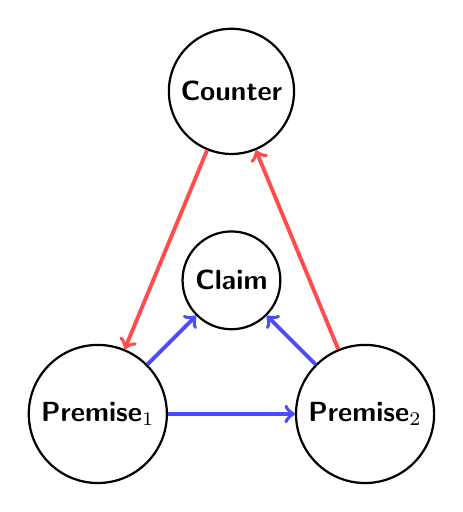
\begin{tikzpicture}[node distance=2.4cm]
        \tikzset{
            arg/.style={draw,circle,thick,minimum size=34pt,font=\sffamily\bfseries},
            support/.style={->, line width=1.4pt, color=blue!70},
            defeat/.style={->, line width=1.4pt, color=red!70}
        }
        \node[arg] (a) {Claim};
        \node[arg] (b) [below left of=a] {Premise$_1$};
        \node[arg] (c) [below right of=a] {Premise$_2$};
        \node[arg] (d) [above of=a] {Counter};
        \draw[support] (b) -- (a);
        \draw[support] (c) -- (a);
        \draw[support] (b) -- (c);
        \draw[defeat] (d) -- (b);
        \draw[defeat] (c) -- (d);
    \end{tikzpicture}
    \caption{Illustrative bipolar argumentation fragment with
             mutual support and derived defeat chains.}
    \label{fig:baf}
\end{figure}

Note that the choice of representing argumentation frameworks in PASP reduces
our problem to performing inference under stable-model semantics with
probabilistic facts. Therefore, any method capable of performing general
inference in PASP is suitable for our purposes.

\section{From Argumentation Mining to PASP}
\label{sec:contribution:pasp}

Argumentation mining systems extract structures such as
Figure~\ref{fig:baf} from text. Early joint models use Integer Linear
Programming to reconcile local classifiers with global constraints
\citep{stab2017parsing}. Probabilistic Logic Programming (PLP) broadens this
perspective: ProbLog enables uncertainty-aware reasoning while preserving
declarative structure \citep{fierens2015inference}. Deep learning can feed
probabilistic choices, as recent neuro-symbolic pipelines demonstrate
\citep{cerveira2023argumentation}.

The Stable-model semantics further increase this expressiveness in PLPs.
The \textsc{smProbLog} system adopts stable-models to handle negative cycles
that may arise in contradictory arguments \citep{totis2023smproblog}. The
literature mostly focuses on stratified programs for tractability, leaving
the probabilistic behaviour of non-stratified encodings largely unexplored. Our
contribution is to develop a pipeline for representating BAFs as PASP programs,
compiling the resulting program into structured circuits that support
efficient inference and that can be translated to automatic differentiation
frameworks, paving the way for scalable neuro-symbolic training loops.

\section{PASP as a 2AMC problem}
\label{sec:pasp_2amc}

The first approach that we consider is the 2AMC problem. This is a generalization of the
AMC problem, superficially described in the literature review
\ref{ch:literature_review} and described in more detail in the
\citep{kimmig2017algebraic, wang2025}. We highly recommend the
reader not familiarized with the WMC problem in general to read
\citep{kimmig2017algebraic} before continuing this section. In
summary, WMC is a framework that generalizes probabilistic inference over
propositional formulas with weighted atoms.

\subsection{Credal Semantics as an Instance of 2AMC}

As described in the preliminary Chapter \ref{ch:pasp}, the
Credal semantics is deeply related to the
notion of \textit{brave} and \textit{cautious reasoning}, in the
sense that we want to compute a probability interval
$[\underline{\mathbb{P}}(\mathcal{M}), \overline{\mathbb{P}}
(\mathcal{M})]$ (Equation \eqref{eq:credal_semantics}), for a set of models
$\mathcal{M}$, such that

$$
\overline{\mathbb{P}}(\mathcal{M}) = \sum_{\theta \in \Theta
: \Gamma(\theta) \cap \mathcal{M} \ne \emptyset} \mathbb{P}
(\theta), \qquad
\underline{\mathbb{P}}(\mathcal{M}) = \sum_{\theta \in
\Theta : \Gamma(\theta) \subseteq \mathcal{M}} \mathbb{P}
(\theta),
$$

where $\Theta$ is the set of all total choices, and $\Gamma
(\theta)$ the set of stable models associated with the
total choice \citep{cozman2017semantics, cozman2020joy}.

Although both equations above are not immediately recognizable
as an instance of the 2AMC problem, its characterization
as:

$$
\overline{\mathbb{P}}(\mathcal{M}) = \sum_{\theta \in \Theta}
\left[ \mathbb{P}(\theta) \cdot \bigwedge_{\gamma \in \Gamma(
\Theta)} [\![ \gamma \in \mathcal{M} ]\!] \right],
$$
$$
\underline{\mathbb{P}}(\mathcal{M}) = \sum_{\theta \in \Theta}
\left[ \mathbb{P}(\theta) \cdot \bigvee_{\gamma \in \Gamma(
\Theta)} [\![ \gamma \in \mathcal{M} ]\!] \right].
$$

Formally, one can see that the two semirings corresponding to
the upper probability interval in a 2AMC problem are:

\begin{itemize}
    \item The inner semiring $\mathcal{S}_I = (\set{0,1},
    \land, \land, \mathrm{true}, \mathrm{true})$, with labeling
    function $\alpha_I$ being constant as \textit{true} for all
    elements of the semiring;
    \item The outer semiring $\mathcal{S}_O = (\mathbb{R}_{\ge
    0}, +, \cdot, 0, 1)$, with labeling function $\alpha_O(o) =
    \mathbb{P}(o)$ for all elements of the semiring, which
    corresponds to the probability of a probabilistic fact $o$.
\end{itemize}

Furthermore, the weight transformation function can be
considered as the identity function, since it corresponds
elements with value $0$ from the inner AMC to $0$ in the
outer AMC, and the same is true for an inner AMC with
value $1$.

A similar approach can be taken for the lower probability, since
the main difference between both \textit{upper} and
\textit{lower} probabilities concerns the notion of
\textit{brave} and \textit{cautious} reasoning, respectively.
Moreover, by applying the ``tuple trick'' \citep{wang2025},
we can create semiring elements capable of representing the
computation of both \textit{upper} and \textit{lower}
probabilities at the same time, as an instance of the
2AMC problem.

\section{Knowledge Compilation Pipeline}
\label{sec:contribution:pipeline}


\begin{equation}
    \textsc{Clark}(P) = \bigwedge_{a \in \mathcal{A}(P)}
    \left[a \iff \bigvee_{r \in \mathcal{R}(P,a)}
    \bigwedge_{b \in \textsc{body}(r)} b
    \bigwedge_{a' \in \textsc{head}(r) \setminus \{a\}} \neg a'
    \right].
    \label{eq:clark_completion_disjunctive}
\end{equation}

Our pipeline grounds a PASP program obtained from a document, applies Clark’s
completion to expose a propositional theory, and then compiles the result into a
probabilistic circuit. Figure~\ref{fig:kc-pipeline} reuses the visual summary
from our poster to emphasise the offline--online separation: expensive
compilation happens once, while inference reuses the circuit.

\begin{figure}[h!]
    \centering
    \begin{tikzpicture}[
        node distance=2.5cm,
        >=Stealth,
        box/.style={rectangle, draw, rounded corners=3pt, line width=0.8pt, align=center},
        data/.style={rectangle, draw, rounded corners=3pt, line width=0.8pt, align=center},
        arrow/.style={->, line width=0.8pt},
        lit/.style={rectangle, draw, rounded corners=2pt, line width=0.6pt, inner sep=2pt, align=center},
        and/.style={circle, draw, line width=0.6pt, inner sep=2pt}
    ]

    % Define x-coordinates for the two columns (Increased for wider spacing)
    \def\ColOneX{0}
    \def\ColTwoX{8.5}
    % Define vertical distance for the bottom row
    \def\BottomRowY{-8}

    % ======================================
    % 1. PASP Program (Top Left)
    % ======================================
    \node[box, fill=green!10, text width=4.5cm, minimum height=4.5cm, anchor=north, align=center] (program) at (\ColOneX, 0) {
        \textbf{PASP Program}
        \begin{minipage}{4cm}
            \vspace{1em}
            \begin{minted}[
                fontsize=\small,
                linenos=false,
                frame=none,
                breaklines
            ]{prolog}
    0.5::stress(X) :- person(X).
    person(turing).
    person(neumann).
            \end{minted}
            \vspace{-0.3em}
        \end{minipage}
    };

    % ======================================
    % 3. Grounded Program (Top Right)
    % ======================================
    \node[data, text width=4.5cm, minimum height=4.5cm, anchor=north, align=center] (grounded_program) at (\ColTwoX, 0) {
        \textbf{Grounded Program}
        \begin{minipage}{4cm}
            \vspace{1em}
            \begin{minted}[
                fontsize=\small,
                linenos=false,
                frame=none,
                breaklines
            ]{prolog}
    0.5::stress(turing).
    0.5::stress(neumann).
            \end{minted}
            \vspace{-0.3em}
        \end{minipage}
    };

    % Draw PASP -> Grounded Program with Grounding label
    \draw[arrow] (program) -- node[midway, above, fill=white, inner sep=2pt] {grounding step} (grounded_program);

    % ======================================
    % 4. Compilation Box with Circuit Inside (Bottom Right)
    % ======================================
    % Main Box
    \node[box, fill=yellow!10, text width=5.5cm, minimum height=4cm, anchor=north] (compilation_box) at (\ColTwoX, \BottomRowY) {};

    % Title placed inside the box, near the top
    \coordinate (compilation_title_center) at ($(compilation_box.north) + (0, -0.2cm)$);
    \node[anchor=north, align=center] (compilation_title) at (compilation_title_center) {\textbf{Compilation}};

    % Draw Circuit inside the Compilation box, positioned 1em below the title
    \begin{scope}[shift={(compilation_box.center)}, yshift=0.5cm]
        % Define nodes for the circuit fragment.
        \node[and, scale=0.7] (p0) at (0, 0) {$\times$};
        \node[and, scale=0.7] (p1) at (-1, -0.7) {$\times$};
        \node[and, scale=0.7] (p2) at (1, -0.7) {$\times$};
        \node[lit] (pt) at (-0.4, -1.7) {$p_t$};
        \node[lit] (st) at (-1.6, -1.7) {$s_t$};
        \node[lit] (pn) at (0.4, -1.7) {$p_n$};
        \node[lit] (sn) at (1.6, -1.7) {$s_n$};

        % Draw connections for the circuit
        \draw[arrow, line width=0.5pt, shorten >= 1pt, shorten <= 1pt] (p0) -- (p1);
        \draw[arrow, line width=0.5pt, shorten >= 1pt, shorten <= 1pt] (p0) -- (p2);
        \draw[arrow, line width=0.5pt, shorten >= 1pt, shorten <= 1pt] (p1) -- (pt);
        \draw[arrow, line width=0.5pt, shorten >= 1pt, shorten <= 1pt] (p1) -- (st);
        \draw[arrow, line width=0.5pt, shorten >= 1pt, shorten <= 1pt] (p2) -- (pn);
        \draw[arrow, line width=0.5pt, shorten >= 1pt, shorten <= 1pt] (p2) -- (sn);
    \end{scope}

    % Draw Grounded Program -> Compilation arrow
    \draw[arrow] (grounded_program.south) -- node[midway, above, fill=white, inner sep=2pt] {rewrite step} (compilation_box.north);

    % ======================================
    % 5. Probabilistic Inference (Bottom Left)
    % ======================================
    \node[data, fill=red!10, text width=4.5cm, minimum height=4cm, anchor=north, align=center] (inference_box) at (\ColOneX, \BottomRowY) {
        \textbf{Probabilistic Inference}
        \begin{minipage}{3.5cm}
            \centering
            \vspace{1em}
            \begin{tabular}{|c|c|}
            \hline
            \textbf{World} & \textbf{P(World)} \\
            \hline
            $\ldots$ & $\ldots$ \\
            \hline
            $s_t, s_n$ & $0.25$ \\
            \hline
            $\neg s_t, \neg s_n$ & $0.25$ \\
            \hline
            \end{tabular}
            \vspace{-0.3em}
        \end{minipage}
    };

    % ======================================
    % 6. Inference Step (Arrow Label)
    % ======================================
    % Draw Compilation -> Probabilistic Inference with Inference Step label
    \draw[arrow] (compilation_box) -- node[midway, above, fill=white, inner sep=2pt] {inference step} (inference_box);

    % ======================================
    % 7. Query Arrow
    % ======================================
    \draw[arrow, densely dashed] (inference_box.north) -- (program.south)
        node[midway, above, fill=white, inner sep=3pt] {query};

    \end{tikzpicture}
    \caption{Knowledge compilation pipeline with grounding, compilation, and
    inference steps.}
    \label{fig:kc_pipeline}
\end{figure}

The compilation stage must accommodate the probabilistic weights attached to
argumentative predicates and the loop formulas required by stable semantics
\citep{cozman2017semantics}. We use the 2AMC formalism to justify correctness
\citep{kiesel2022efficient} and adopt existing optimisations that control the
number of auxiliary variables introduced during completion
\citep{EITER2024104109}.

\section{Structured Circuits for Tractable Inference}
\label{sec:contribution:circuits}

The target circuits obey three structural properties that make weighted model
counting tractable \citep{Darwiche_2002, darwiche2011sdd}:
\begin{itemize}
    \item \textbf{Decomposability}: sub-circuits combined by a product node refer
          to disjoint sets of variables.
    \item \textbf{Determinism}: the children of a sum node are mutually
          exclusive, preventing double counting.
    \item \textbf{Smoothness}: the children of a sum node mention the same
          variables, enabling weight sharing and differentiation.
\end{itemize}

\begin{figure}[ht]
    \centering
    \begin{tikzpicture}[scale=1.05, every node/.style={font=\small}]
        \tikzset{
            sum/.style={draw,circle,thick,line width=1pt,inner sep=3pt,color=cyan!70!black},
            and/.style={draw,circle,thick,line width=1pt,inner sep=3pt,color=orange!80!black},
            lit/.style={font=\small\ttfamily}
        }
        \node[sum] (root) at (0,0) {$+$};
        \node[and] (and1) at (-2,-1.6) {$\times$};
        \node[and] (and2) at (2,-1.6) {$\times$};
        \node[sum] (sum1) at (-3.4,-3.2) {$+$};
        \node[lit] (litb) at (-0.6,-3.2) {$b$};
        \node[lit] (lita) at (-4.5,-4.8) {$a$};
        \node[lit] (litna) at (-2.3,-4.8) {$\neg a$};
        \node[lit] (litc) at (1.2,-3.2) {$a$};
        \node[lit] (litnb) at (3.0,-3.2) {$\neg b$};
        \draw (root) -- (and1);
        \draw (root) -- (and2);
        \draw (and1) -- (sum1);
        \draw (and1) -- (litb);
        \draw (sum1) -- (lita);
        \draw (sum1) -- (litna);
        \draw (and2) -- (litc);
        \draw (and2) -- (litnb);
    \end{tikzpicture}
    \caption{Smooth, decomposable, and deterministic circuit fragment used for
             PASP inference.}
    \label{fig:structured-circuit}
\end{figure}

Figure~\ref{fig:structured-circuit} highlights how the properties arise in
practice: the left branch considers two mutually exclusive cases for $a$ before
combining them with evidence about $b$, while the right branch enforces a
complementary scenario. These circuits support linear-time evaluation for
evidence updates and can be differentiated to align neural predictions with the
logical structure.

\section{Experimental Results}
